\section{DF model dynamics} 
% FOR ALL FORCES: 
    % define them 
    % explain how they get computed 
% Show a simulation run with all forces combined 
% also explained the numerical solver and method that gets used 


\paragraph{Area force}

\begin{proposition}  \textbf{Shoelace formula for DF cells} \label{prop:Shoelace}\\ 
	Let $C = (\vec{x}_1, \ldots, \vec{x}_N)$ be a positively orientated DF cell with $\vec{x}_i = (x_i, y_i)^T$.
	Then, the area $A_C$ of $C$ can be determined through the shoelace formula
	\begin{center}
		$A_C = \frac{1}{2}\sum\limits_{i = 1}^{N} (x_i y_{i+1} - x_{i+1} y_i)$,
	\end{center} 
	where $\vec{x}_{N + 1} := \vec{x}_1$. \\
	Proof. 	\\
	An illustration of the proof is given in Figure \ref{fig:shoelace}, which is where the idea of the proof comes from. We can assume without the loss of generality that all coordinates are positive. Otherwise we could move the figure in the positive coordinate directions until all entries are positive without changing the area. \\
	For every $1 \leq i \leq N$ the edge $\overline{ \vec{x}_i \: \vec{x}_{i+1}}$ gets assigned to the area $T_i$ of the trapeze that arises when one connects the line segment vertically with the $x$ axis. We get
	\begin{center}
		$T_i = \frac{1}{2} (y_i + y_{i+1})(x_i - x_{i+1})$.
	\end{center}
	Keep in mind that $\vec{x}_{N + 1} := \vec{x}_1$. \\
	The area $T_i$ has a positive sign if $x_i \geq x_{i+1}$ (green arrow in Figure \ref{fig:shoelace}) and a negative sign otherwise (red arrow). As one can see in the figure, the negatively signed $T_i$'s take up exactly the areas that are superfluous if one just adds all the positive $T_i$'s. 
	Thus the total polygon's area is equal to the sum of all trapezes
	\begin{center}
		$A_C = \sum\limits_{i = 1}^{N} T_i = \frac{1}{2} \sum\limits_{i = 1}^{N} (y_i + y_{i+1})(x_i - x_{i+1}) = \frac{1}{2}\sum\limits_{i = 1}^{N} (x_i y_{i+1} - x_{i+1} y_i) $.
	\end{center} 
	\begin{figure}[h!]
		\begin{center}
			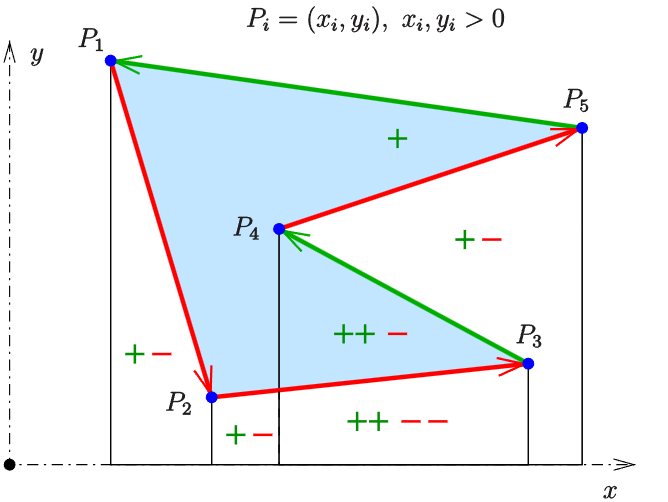
\includegraphics[width=8cm]{shoelace.png}
			\caption{
				This figure shows a geometrical interpretation of the shoelace formula. In difference to the proposition, here the vertices are called $P_i$ and not $\vec{x}_i$. \\
				Source: \cite{ShoelaceFigure2022}}
			\label{fig:shoelace}
		\end{center}
	\end{figure}
	\qed
\end{proposition}

\paragraph{Edge force}

\paragraph{Interior angle force}

\paragraph{Overlap force}
% explain the algorithm

\subsection{A simulation run}
% state the force system
% DifferentialEquations.jl solver \\
%  -> Euler Maruyama method with fixed time step size  \\